%% LyX 2.0.8.1 created this file.  For more info, see http://www.lyx.org/.
%% Do not edit unless you really know what you are doing.
\documentclass{IEEEtran}
\usepackage[latin9]{inputenc}
\usepackage[letterpaper]{geometry}
\geometry{verbose,tmargin=1in,bmargin=1in,lmargin=1in,rmargin=1in}
\setlength{\parskip}{\smallskipamount}
\setlength{\parindent}{0pt}
\usepackage{color}
\usepackage{float}
\usepackage{textcomp}
\usepackage{url}
\usepackage{graphicx}
\usepackage[unicode=true,pdfusetitle,
 bookmarks=true,bookmarksnumbered=false,bookmarksopen=false,
 breaklinks=true,pdfborder={0 0 0},backref=false,colorlinks=true]
 {hyperref}
\hypersetup{
 linkcolor=blue,urlcolor=blue,citecolor=blue}

\makeatletter
%%%%%%%%%%%%%%%%%%%%%%%%%%%%%% User specified LaTeX commands.
\usepackage{color}%% maxwidth is the original width if it is less than linewidth
%% otherwise use linewidth (to make sure the graphics do not exceed the margin)

\def\maxwidth{ %
  \ifdim\Gin@nat@width>\linewidth
    \linewidth
  \else
    \Gin@nat@width
  \fi
}


\definecolor{fgcolor}{rgb}{0.2, 0.2, 0.2}
\newcommand{\hlnumber}[1]{\textcolor[rgb]{0,0,0}{#1}}%
\newcommand{\hlfunctioncall}[1]{\textcolor[rgb]{0.501960784313725,0,0.329411764705882}{\textbf{#1}}}%
\newcommand{\hlstring}[1]{\textcolor[rgb]{0.6,0.6,1}{#1}}%
\newcommand{\hlkeyword}[1]{\textcolor[rgb]{0,0,0}{\textbf{#1}}}%
\newcommand{\hlargument}[1]{\textcolor[rgb]{0.690196078431373,0.250980392156863,0.0196078431372549}{#1}}%
\newcommand{\hlcomment}[1]{\textcolor[rgb]{0.180392156862745,0.6,0.341176470588235}{#1}}%
\newcommand{\hlroxygencomment}[1]{\textcolor[rgb]{0.43921568627451,0.47843137254902,0.701960784313725}{#1}}%
\newcommand{\hlformalargs}[1]{\textcolor[rgb]{0.690196078431373,0.250980392156863,0.0196078431372549}{#1}}%
\newcommand{\hleqformalargs}[1]{\textcolor[rgb]{0.690196078431373,0.250980392156863,0.0196078431372549}{#1}}%
\newcommand{\hlassignement}[1]{\textcolor[rgb]{0,0,0}{\textbf{#1}}}%
\newcommand{\hlpackage}[1]{\textcolor[rgb]{0.588235294117647,0.709803921568627,0.145098039215686}{#1}}%
\newcommand{\hlslot}[1]{\textit{#1}}%
\newcommand{\hlsymbol}[1]{\textcolor[rgb]{0,0,0}{#1}}%
\newcommand{\hlprompt}[1]{\textcolor[rgb]{0.2,0.2,0.2}{#1}}%

\usepackage{framed}
\newenvironment{kframe}{%
 \def\at@end@of@kframe{}%
 \ifinner\ifhmode%
  \def\at@end@of@kframe{\end{minipage}}%
  \begin{minipage}{\columnwidth}%
 \fi\fi%
 \def\FrameCommand##1{\hskip\@totalleftmargin \hskip-\fboxsep
 \colorbox{shadecolor}{##1}\hskip-\fboxsep
     % There is no \\@totalrightmargin, so:
     \hskip-\linewidth \hskip-\@totalleftmargin \hskip\columnwidth}%
 \MakeFramed {\advance\hsize-\width
   \@totalleftmargin\z@ \linewidth\hsize
   \@setminipage}}{\par\unskip\endMakeFramed%
 \at@end@of@kframe}



\definecolor{messagecolor}{rgb}{0, 0, 0}
\definecolor{warningcolor}{rgb}{1, 0, 1}
\definecolor{errorcolor}{rgb}{1, 0, 0}
\newenvironment{knitrout}{}{} % an empty environment to be redefined in TeX

\usepackage{alltt}\usepackage{booktabs}\usepackage{fullpage}



% Create a new command, \blfootnote which creates a footnote without a number
\newcommand{\blfootnote}[1]{%
  \begingroup
  \renewcommand\thefootnote{}\footnote{#1}%
  \addtocounter{footnote}{-1}%
  \endgroup
}
\IfFileExists{upquote.sty}{\usepackage{upquote}}{}

\makeatother

\begin{document}

\title{{\small{}Guam New Invasive Species Alert No. 2016-01}\\
 {\Huge{}Greater Banded Hornet}{\huge{}}\\
{\huge{} }\textit{\huge{}Vespa tropica}\\
 {\huge{}(Hymenoptera: Vespidae) }}


\author{Christopher A. Rosario, Lee Roy Sablan, Ross H. Miller, and Aubrey
Moore\\
 University of Guam, College of Natural and Applied Sciences\\
 July 13, 2016\\
Updated August 19, 2016}

\maketitle
\begin{figure}[H]
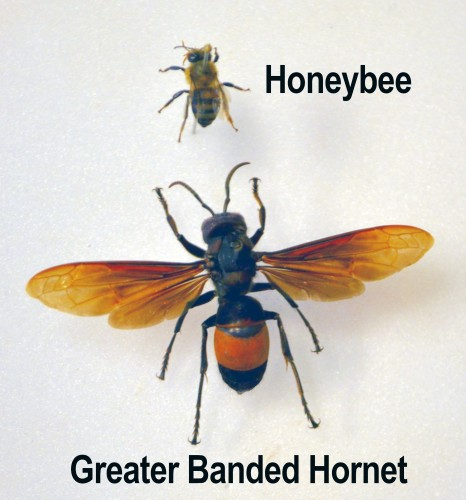
\includegraphics[width=1\columnwidth]{Hornet_bee500} \protect\caption{\label{fig:vespa-tropica}The first greater banded hornet collected
on Guam with a honeybee for size comparison. Photo by Olympia Terral. }
\end{figure}


On July 12, 2016, University of Guam research assistant Christopher
Rosario discovered a colony of large wasps nesting in a hollow avocado
tree in Dededo, Guam (13.50533� N, 144.80134� E). The wasps were aggressive,
resulting in only a single specimen being collected. This observation
was posted on the iNaturalist web site (\url{http://www.inaturalist.org/observations/3663868}).

On July 20, 2016, Arnold Perez of the Leo Palace Resort delivered
5 specimens of \textit{Vespa tropica} to Dr. Aubrey Moore at the University
of Guam. Perez discovered a nest near a swiiming pool (\url{http://www.inaturalist.org/observations/3710757}).
Specimens were placed in the University of Guam Insect Collection.

A press release was issued requesting residents of Guam to report
sightings of \emph{V. tropica}. These sightings are being documented
in an iNaturalist project set up for this purpose (\url{http://www.inaturalist.org/projects/vespa-tropica-on-guam}). 


\section*{Description}

UOG entomologists (Sablan and Moore) identified the wasp as \textit{Vespa
tropica} based on publicly available images and keys \cite{archer1991taxonomy}.
This species determination was confirmed by Dr. Jason Mottern at the
USDA Systematic Entomology Laboratory.

\emph{Vespa tropica} is a medium-sized to large species. Queens reach
30mm or more, males average 26mm and workers average 24 to 26mm.

The nest of \textit{Vespa tropica} is usually underground or in a
tree hollow or similar enclosed space. Due to the location, the nest
is seldom seen. If excavated, the nest usually appears rhomboid or
bowl-shaped, with an open bottom (as opposed to the completely sealed
nests of most aerial hornets). The nest envelope is laminar (comprising
of distinct, broad individual layers) and very brittle.


\subsection*{Human Health Risk}

\emph{V. tropica} is very aggressive and readily stings in the vicinity
of its nest. Death caused by the venom from multiple stings from this
species has been documented, but this is very rare. As with any stinging
insect, an allergic reaction (anaphylaxis) is far more dangerous.
About 3\% of adults are allergic to insect stings \cite{golden2007insectsting}
.


\subsection*{Environmental and Agricultural Risk}

This species is known to attack the nests of Polistines (paper wasps)
in order to obtain the larvae to feed their own larvae. On Guam, a
video recording has been made by Wayne Borja which documents \emph{V.
tropica} raiding a \emph{Polistes stigma} nest, one of 2 species of
small paper wasps locally referred to as ''boonie bees'' (\url{https://www.youtube.com/watch?v=gVXR44ixrxk}).
\emph{V. tropica} has also been reported to raid hives of the European
honeybee, \emph{Apis mellifera} \cite{burgett1982predation}.

\begin{figure}
\includegraphics[width=1\columnwidth,height=1\textheight,keepaspectratio]{\string"Screenshot from 2016-08-19 13:36:39\string".png}

\caption{\emph{\label{fig:Vespa-tropica-sightings}Vespa tropica} sightings
to date.}


\end{figure}



\section*{Geographic Distribution}


\subsection*{Global Distribution}

\textit{Vespa tropica} is found in China, Japan, Malaysia, Hong Kong,
Singapore, India, and the Philippines \cite{GBIF}.


\subsection*{Guam Distribution}

To date, there have been eleven sightings of \emph{V. tropica}, all
in central Guam (Fig. \ref{fig:Vespa-tropica-sightings}).


\section*{Control Recommendations}

The Guam distribution of \emph{V. tropica} indicates that island-wide
eradication is not feasable. If a \emph{V. tropica} nest is discovered,
it should be left alone unless it is in a high risk area such as immediately
adjacent to a home or school. Nest removal is dangerous and should
be attempted only by experienced pest control operators.

\bibliographystyle{plainnat}
\bibliography{VespaTropica}

\end{document}
